\section{Problem Statement and outline}
Particle colliders such as the LHC grant insight into physics by
creating heavy short lived particles that do not occur without a high energy collision
and only persist for a fraction of a second before decaying into lighter particles.
There is then a sequence of decays, known as a shower, before something
stable and long live enough to reach the detectors is created.
From the remnants of the decay that reach the detector we seek
to characterise the heavy particle created in the collision.

The data pipeline can be seen as a whole in~\cite{Stoye_DeepCMS2018, Schramm:2291608}.
Evidence of the shower is gathered from multiple concentric detectors about the collision point, the primary components being the 
silicon tracker for charged particles and the calorimeter for neutral particles. 
These can be seen in figure~\ref{fig:lit_CMSdetector}.
\begin{figure}
    \centering
    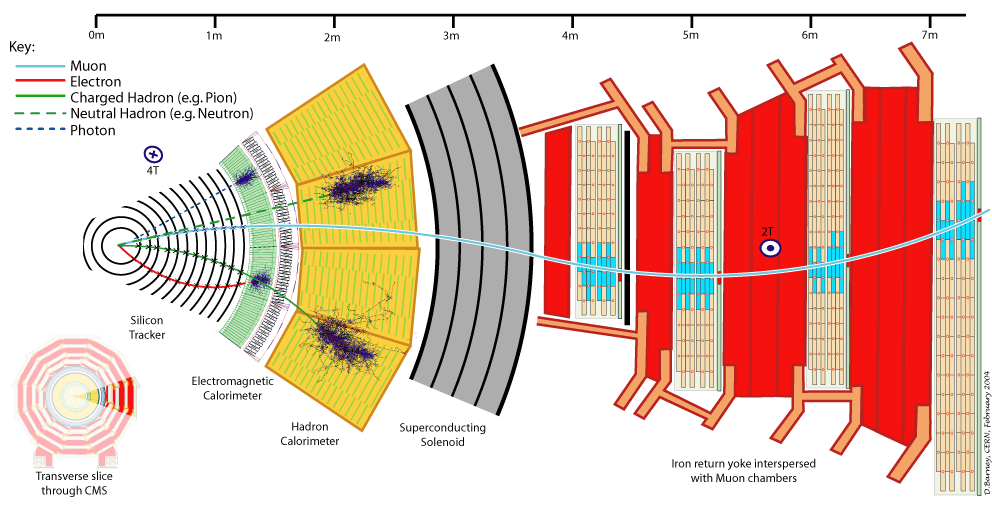
\includegraphics[width=0.8\textwidth]{images/lit_CMSdetector.png}
    \caption{The CMS detector has a concentric structure with each layer sensitive to a subset of possible particles.
             \cite{Stoye_DeepCMS2018}}
             % ADD could add more to this caption
    \label{fig:lit_CMSdetector}
\end{figure}
This data is essentially a series of energy deposits associated with three dimensional coordinates,
there is no time stamp available because the interaction occurs faster than the electronics can read out.
At this point the Particle Flow algorithm is used to reconstruct four vector tracks from the readings~\cite{Beaudette_particleFlow2013}.

%A signal of particular interest is found in the extended Higgs sector.
%Since the discovery of the Higgs Boson in 2012, it's couplings
%have been seen to be in agreement with the Standard Model (SM),
%however additional Higgs particles remain possible.
%The second doublet of the 2HDM allows a further 5 particles;
%two CP even (\(h\) and \(H\), with, conventionally, \(m_h < m_H\)),
%one CP odd (\(A\))
%and a pair of charged (\(H^\pm\)) Higgs bosons.
One possibility under investigation in these experiments is that of an extended Higgs sector
such as the two Higgs Doublet model (2HDM)~\cite{Branco2012THDM}.
The 2HDM introduces 5 new particles;
two CP even (\(h\) and \(H\), with, conventionally, \(m_h < m_H\)),
one CP odd (\(A\))
and a pair of charged (\(H^\pm\)) Higgs bosons.
These come about from the addition of two complex scalar doublets \(\Phi_{1,2}\) from \(SU(2)_L\) with 
the most general gauge invariant renormalisable scalar potential given by:
\begin{align}\nonumber
V(\Phi_1,\Phi_2) =& m_{11}^2\Phi_1^\dagger\Phi_1+m_{22}^2\Phi_2^\dagger\Phi_2-[m_{12}^2\Phi_1^\dagger\Phi_2+{\rm h.c.}] \nonumber
\end{align}
\begin{align}
+& \frac{\lambda_1}{2}(\Phi_1^\dagger\Phi_1)^2
+\frac{\lambda_2}{2}(\Phi_2^\dagger\Phi_2)^2
+\lambda_3(\Phi_1^\dagger\Phi_1)(\Phi_2^\dagger\Phi_2)\nonumber\\
+&\lambda_4(\Phi_1^\dagger\Phi_2)(\Phi_2^\dagger\Phi_1) 
+\frac{1}{2}[\lambda_5~(\Phi_1^\dagger\Phi_2)^2 +~{\rm h.c.}]\nonumber\\
+&\big[ (\lambda_6(\Phi_1^\dagger\Phi_1)
+\lambda_7(\Phi_2^\dagger\Phi_2))
\Phi_1^\dagger\Phi_2+{\rm h.c.}\big] \,. \label{pot1}
\end{align}
Following the hermiticity of the scalar potential, \(m_{11}^2\), \(m_{22}^2\) and \(\lambda_{1,\ldots4}\) are real parameters
whereas \(m_{12}^2\), \(\lambda_{5,6,7}\) can be complex.
Assuming the CP-conserving version of the 2HDM, \(m_{12}^2\), \(\lambda_{5,6,7}\) and the VEVs of the fields \(\Phi_i\) are real parameters.
As a consequence of extending the discrete \(Z_2\) symmetry to the Yukawa sector in order to avoid Flavour Changing Neutral Currents (FCNCs) at tree level,
\(\lambda_{6,7}=0\), whereas the mass term \(m_{12}^2\) breaks the symmetry in a soft way.

Amongst the many signals that these additional Higgs states could produce,
of particular relevance are those involving their cascade decays,
wherein a heavier Higgs state decays in a pair of lighter ones or else into a light Higgs state and a gauge boson.
This is the case as the former process gives access to the shape of the Higgs potential of the enlarged Higgs sector
while the latter channel is intimately related to the underlying gauge structure, which may well be larger than the SM one. 
The focus of these investigations is the use of decay cascades involving Higgs bosons (either amongst themselves or in association to gauge bosons) in order to understand both the Higgs potential and gauge structure which may exist beyond the SM.
%The focus is tools that form and classify jets in challenging topologies.
%Such topologies represent hard to access areas of many predictions, such as those of the Two Higgs Doublet Model (2HDM).
%Tools that were able to utilise more of the information held in the data generated by high energy experiments, such as those at the LHC,
%might be able to exclude or confirm the present of multiple Higgs like particles.

The first part of this investigation will extend and recast the bounds on
2HDM model parameters.
The aim being to identify model parameters that there is sensitivity to after the next LHC upgrade.
Existing scans were also recast to look at alternative decay channels.

The second part of this investigation looks at the best use of existing tools
to process this signal.
In particular the optimal way to cluster particles into jets.

In a detector, jet clustering is designed to aid reconstruction of decayed particles.
The default choice for jet clustering tends to be one of three algorithms;
the anti-kt algorithm~\cite{Cacciari2008akt}, the Cambridge-Aachen algorithm~\cite{Wobisch1998caJet} and the kt algorithm~\cite{Ellis1993ktJet}.
These algorithms are often turned to as they are infrared safe, excellent implementations of them are available (see \fastjet{}~\cite{Cacciari2011FastJet})
and they are flexible enough to capture many signals with minimal parameter change.

For a cascade decay in a 2HDM model this process presents a particular challenge owing to the
mass difference between the \bthing{quark} and heavy Higgs.
The decays tend to be collimated and the jets often merge or overlap.

Finally there is an investigation of possible machine learning inspired jet clustering techniques.
A recursive algorithm is well suited to clustering objects when the number of groups is not known at outset.
Agglomerative algorithms are easier to design in a manner that is infrared safe,
as they can recombine soft and collinear emissions in early steps.
Spectral clustering is considered as it can be performed in a recursive agglomerative manner.


%Once the jets have been formed it then remains to identify the decayed tag particle they represent.
%The tag particle is the particle that leaves the hard interaction, or is immediately descendant of the proton beam,
%that decays to form the shower.
%There are a number of factors effecting the difficulties of identifying this particle.
%One of these would be how well the shower has been isolated by the jet.
%Sometimes two showers overlap strongly, so one jet in fact contains the combination of two showers,
%identifying both originating particles together is especially challenging.
%This is often the case when a very high energy particle decays into lighter particles,
%and the descendants have high kinetic energy, which sends them in a boosted configuration as a shallow angle to the beam line.
%
%
%This is relevant to jet physics because the additional Higgs particles most commonly to decay to \bthing{quarks} which shower to form jets.
%These jets may have a highly boosted configuration due to the mass difference between the \bthing{quark} and the heavy Higgs.
%As such the 2HDM is a prime example of the types of signals that might benefit from advances in jet formation and classification.
